\documentclass{standalone}
\usepackage{tikz}
\usepackage{amsmath}
\usepackage{pgfplots}
\usepackage{xcolor}
\definecolor{Yellow}{rgb}{1,0.75,0.1}
\pgfplotsset{compat=1.17} % Adjust if needed

\begin{document}

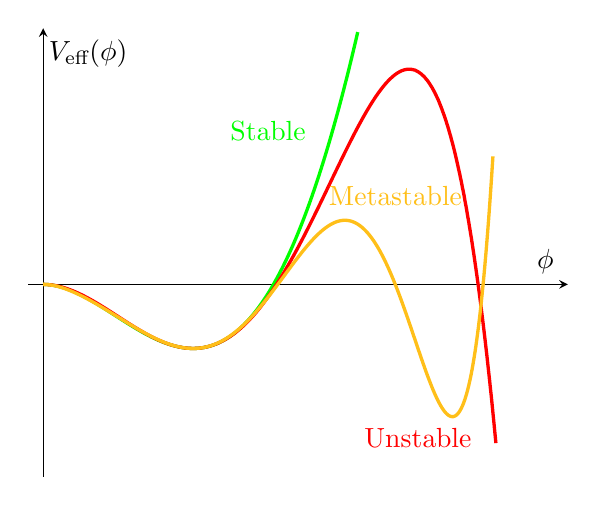
\begin{tikzpicture}
  \begin{axis}[
    samples=500,
    domain=-0.1:8,
    xmin=-0.1, xmax=3.5,
    ymin=-1.5, ymax=2,
    axis lines=middle,
    restrict y to domain=-2:2,
    restrict x to domain=-0.1:3.1,
    xtick=\empty,                % Remove x-axis ticks
    ytick=\empty,        % Remove y-axis ticks
    legend style={draw=none,     % Hide box around legend
                  at={(0.5,0.95)},
                  anchor=north,
                  legend cell align={left}}
  ]
    % Green curve
    \addplot[
      very thick,
      color=green,
      domain=0:3
    ]
    plot (\x, {-1.625*x^2 + 1.25*x^3 - 0.125*x^4});

    % Red curve
    \addplot[
      very thick,
      color=red,
      domain=0:3.02
    ]
    plot (\x, {(-13*x^2)/9 + (53*x^3)/72 + (13*x^4)/36 - (11*x^5)/72});

    % Yellow curve
    \addplot[
      very thick,
      color=Yellow,
      domain=0:3
    ]
    plot (\x, {-1.9883333333333377*x^2
               + 3.217037037037059*x^3
               - 3.9490740740741126*x^4
               + 3.3944444444444746*x^5
               - 1.3681481481481588*x^6
               + 0.19407407407407548*x^7});
  \node[color=green] at (1.5,1.2) {Stable};
  \node[color=red] at (2.5,-1.2) {Unstable};
  \node[color=Yellow] at (2.35,0.69) {Metastable};
  \node[color=black] at (0.3,1.8) {$V_{\text{eff}}(\phi)$};
  \node[color=black] at (3.35,0.18) {$\phi$};
  \end{axis}

\end{tikzpicture}

\end{document}